In this part, we using \emph{Out of Place} measurement to date the article by two different kind of approaches (i.e., whether use unmatched word or not). See figure \ref{outofplace_1840_all}, \ref{outofplace_1840_match},\ref{outofplace_1960_all}, \ref{outofplace_1960_match}, \ref{outofplace_1995_all} and \ref{outofplace_1995_match} for more details.

\begin{figure}[H]
    \begin{minipage}[b]{0.48\linewidth}
        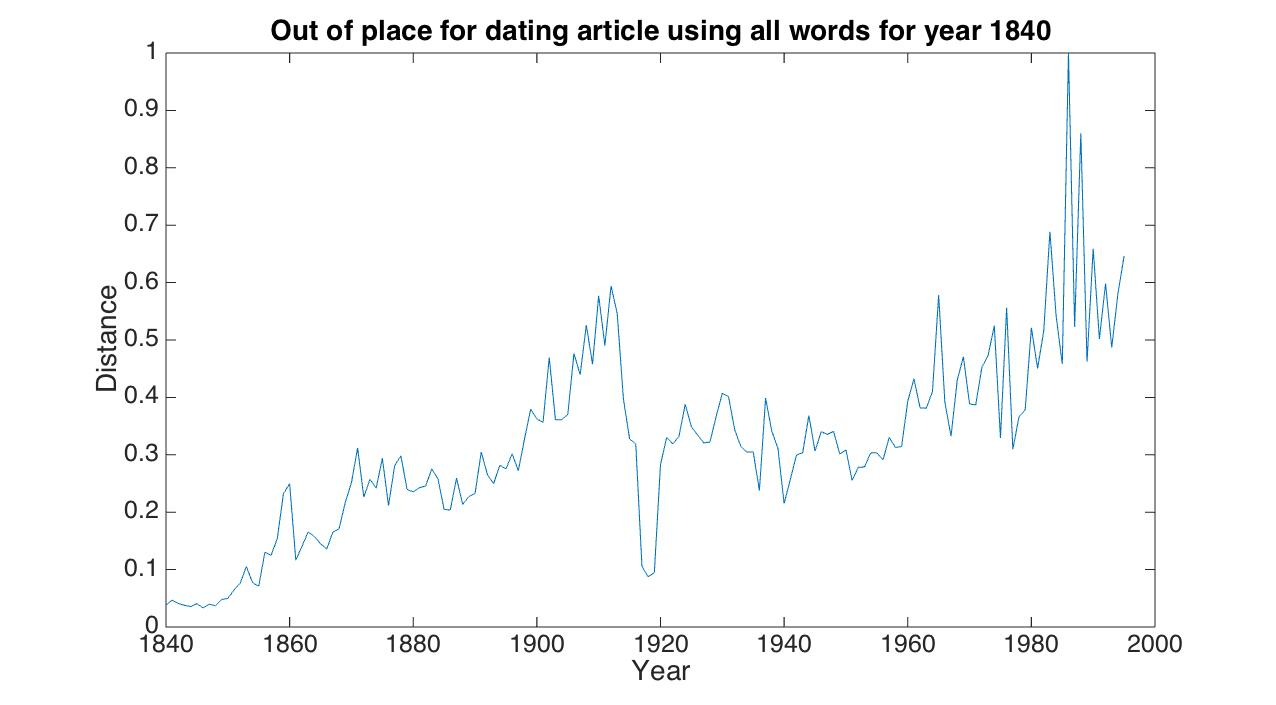
\includegraphics[scale=0.15]{Pictures/date_articles/outofplace/1840_all.jpg}
        \caption{Out of place for dating article using all words for year 1840}
        \label{outofplace_1840_all}
    \end{minipage}\hfill
    \begin{minipage}[b]{0.5\linewidth}
        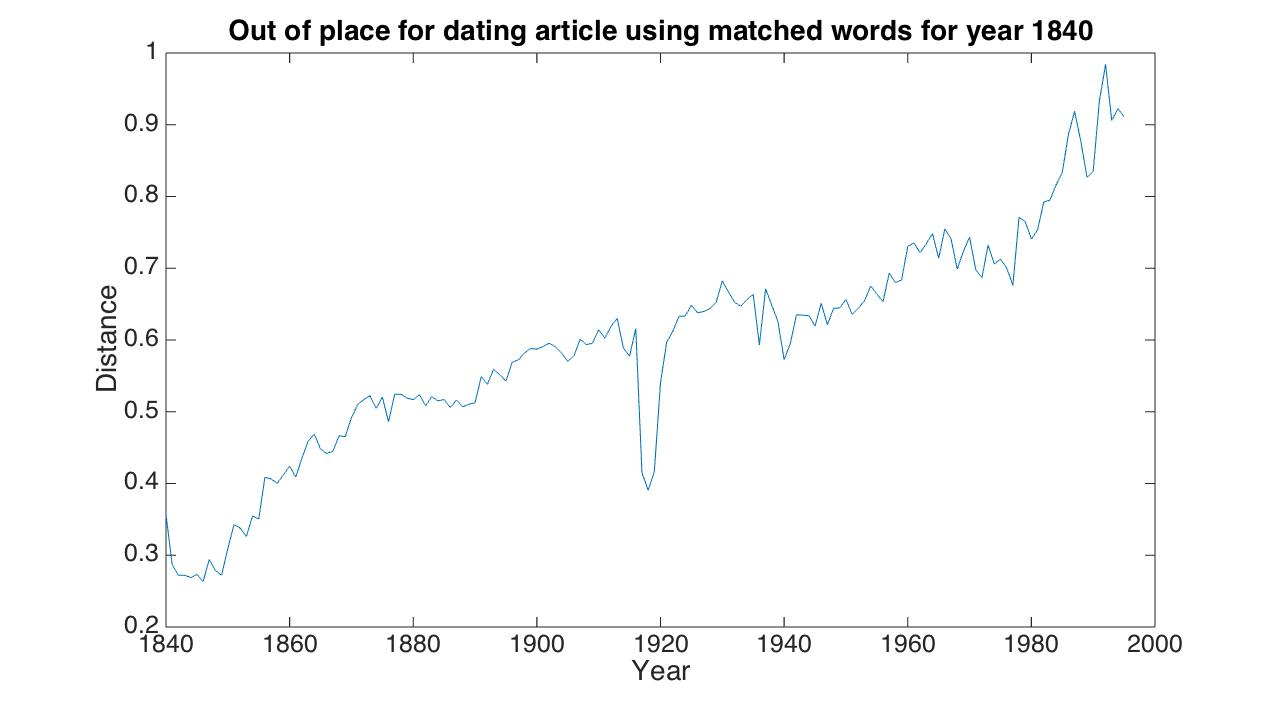
\includegraphics[scale=0.15]{Pictures/date_articles/outofplace/1840_partial.jpg}
        \caption{Out of place for dating article using matched words for year 1840}
        \label{outofplace_1840_match}
    \end{minipage}\hfill
\end{figure}

\begin{figure}[H]
    \begin{minipage}[b]{0.48\linewidth}
        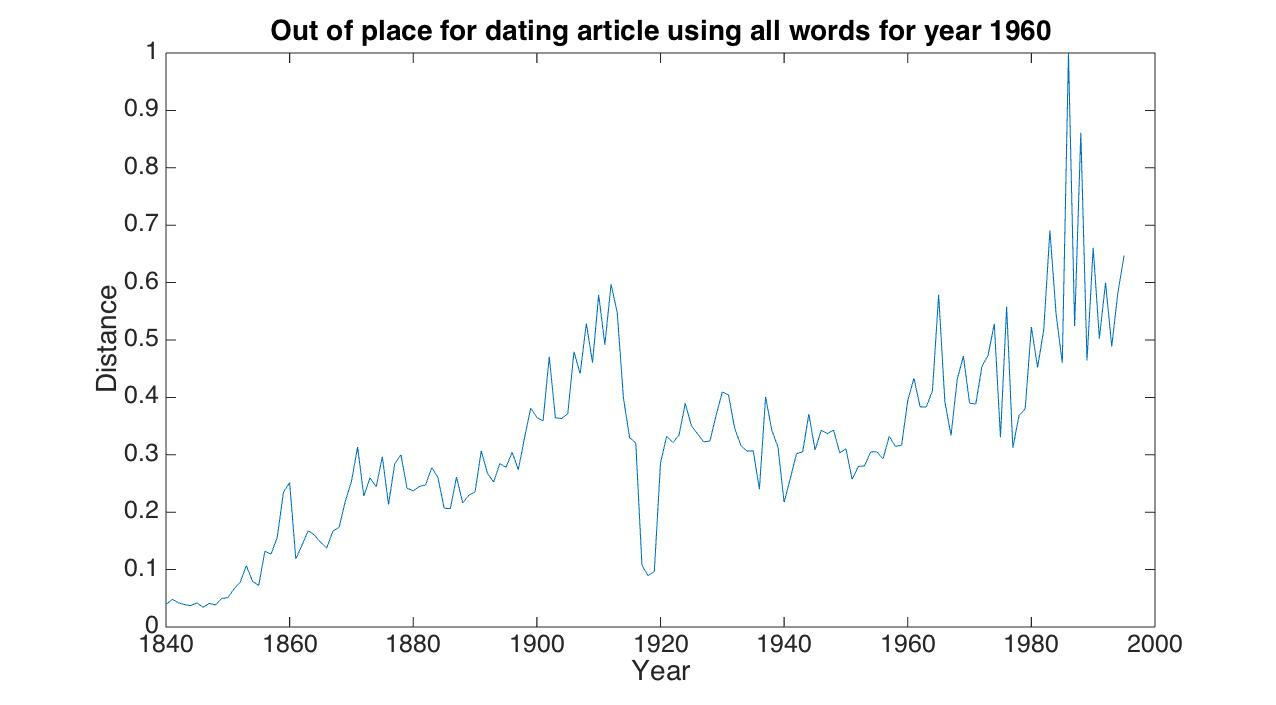
\includegraphics[scale=0.15]{Pictures/date_articles/outofplace/1960_all.jpg}
        \caption{Out of place for dating article using all words for year 1960}
        \label{outofplace_1960_all}
    \end{minipage}\hfill
    \begin{minipage}[b]{0.5\linewidth}
        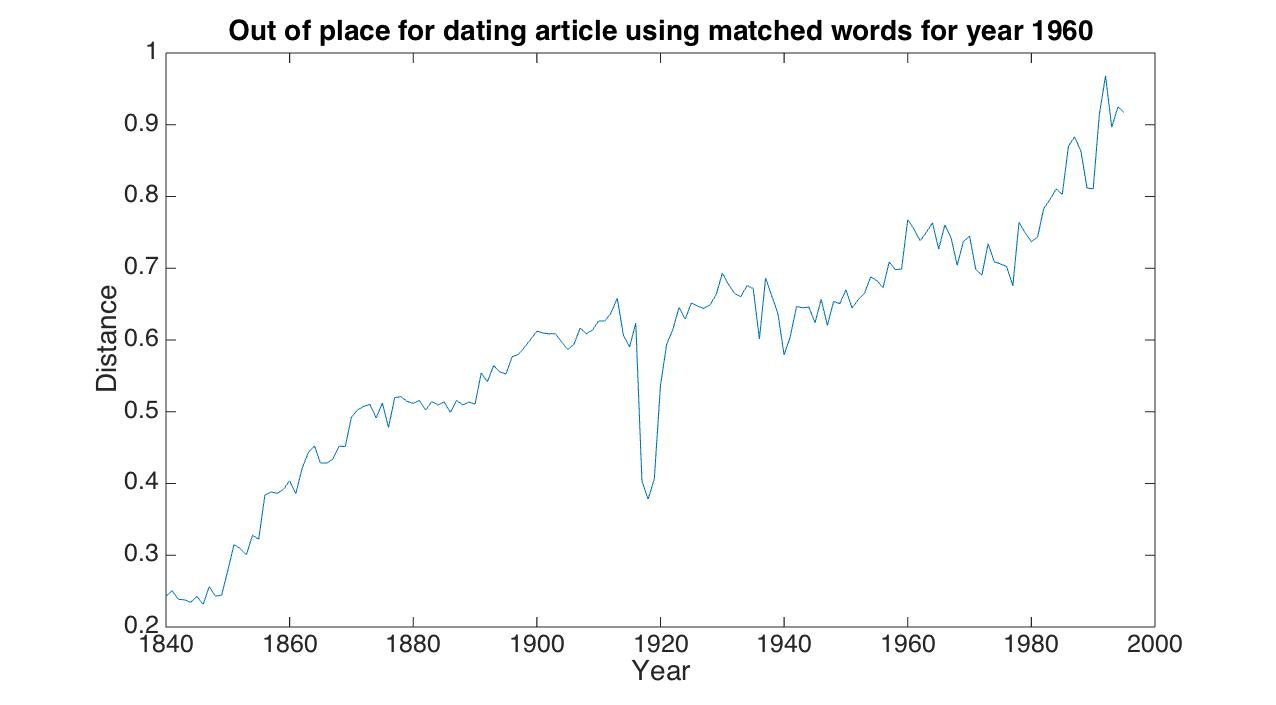
\includegraphics[scale=0.15]{Pictures/date_articles/outofplace/1960_partial.jpg}
        \caption{Out of place for dating article using matched words for year 1960}
        \label{outofplace_1960_match}
    \end{minipage}\hfill
\end{figure}

\begin{figure}[H]
    \begin{minipage}[b]{0.48\linewidth}
        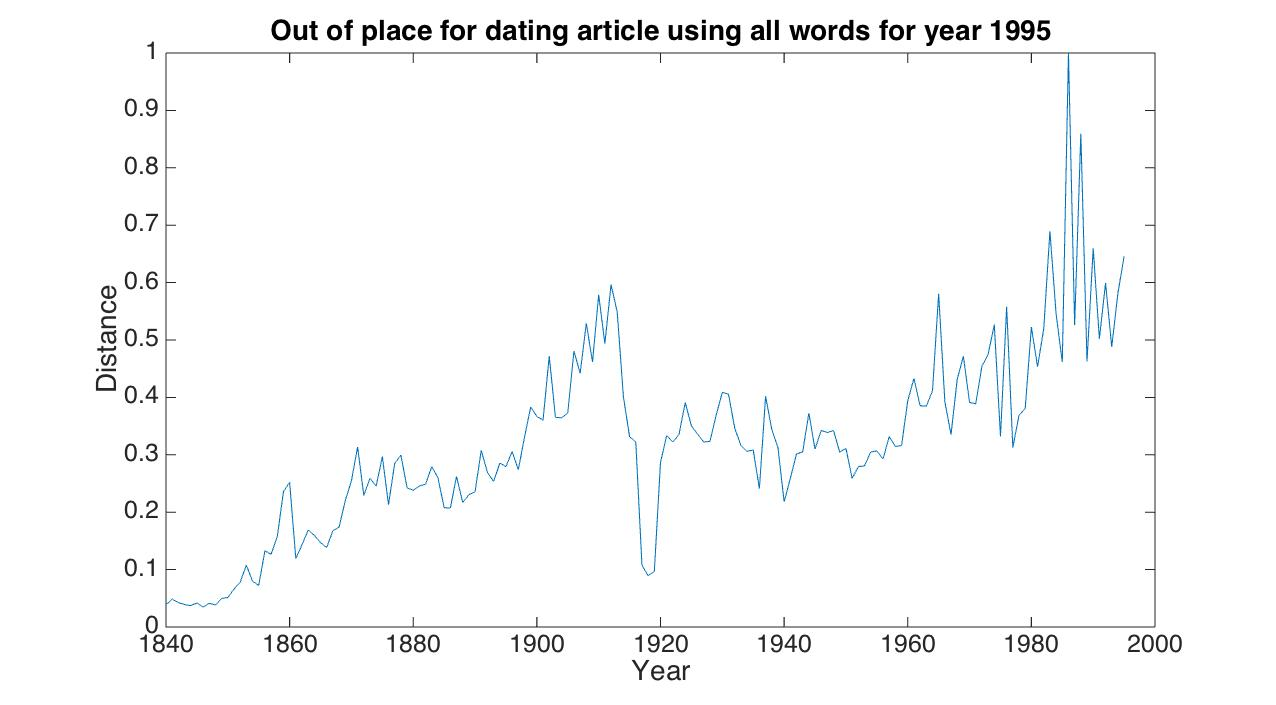
\includegraphics[scale=0.15]{Pictures/date_articles/outofplace/1995_all.jpg}
        \caption{Out of place for dating article using all words for year 1995}
        \label{outofplace_1995_all}
    \end{minipage}\hfill
    \begin{minipage}[b]{0.5\linewidth}
        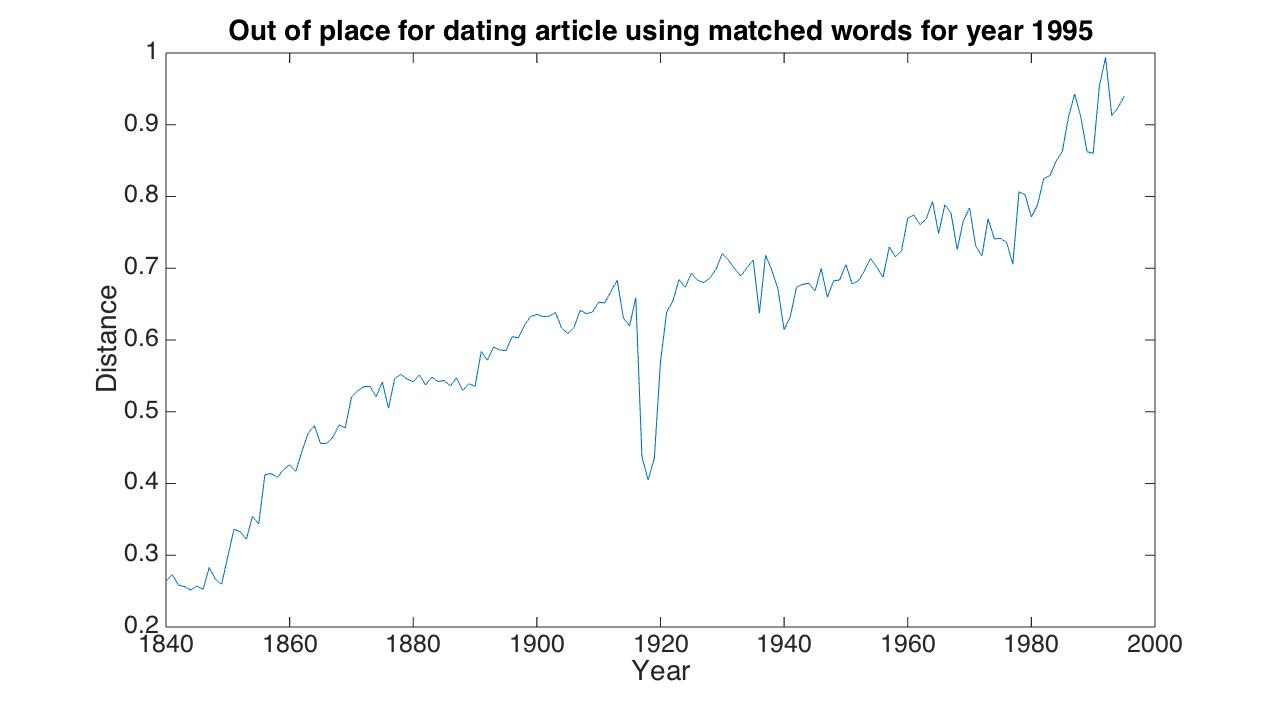
\includegraphics[scale=0.15]{Pictures/date_articles/outofplace/1995_partial.jpg}
        \caption{Out of place for dating article using matched words for year 1995}
        \label{outofplace_1995_match}
    \end{minipage}\hfill
\end{figure}

If we only look at the result of year $1840$, we can say that it is a good metric for its high-accuracy of prediction. However, when tracking the condition on other years, the result is really odd since all of them give a same plot if we just classify them by eyes. Check its detailed information, there exists a slight difference between different pairs of article and years for the \emph{Out of Place} measurement. However, we cannot deny that it works bad on dating article.

Returning to the formula of \emph{Out of Place} measurement and also considering the size of article, this odd phenomenon then can be explained. For dating article, we only randomly select 15 articles whose size is too small to affect the rank of words that appears in the year data even though we have already removed word's frequency of article from the year it belongs to. As a result, noises are introduced to the final result or useful information are missing.

If we use all words, due to the big gap between the size of article and years, valuable information will be hidden by large volume noises which explains the unchangeable phenomenon on the distance of different article and years. If we only use matched words, for articles that from different years, the matched words are greatly limited by the year data, thus the computation process will always happen on the similar article dataset and year dataset if article data varies but year data remains the same. That is why the \emph{Out of Place} measurement met some changes among part of relationships but still remain a similar trend.

Thus, as explained above, the \emph{Out of Place}, at least for the function of dating article, is not a good metric.

